\ifx\wholebook\relax\else
\input{../Common.tex}
\input{../macroes.tex}
\begin{document}
\fi

\chapter{Errors and Debugging}\label{ch:debugger}

Now that you know how to define methods calling other methods, it is time to have a look at a really powerful tool that helps you to find your errors: the \sq debugger. A debugger is a tool that presents  the execution of a program and lets you inspect and changes the values of the variables or the methods of a program. Therefore in this chapter I will present some possible errors and what is a debugger. I start to present some errors you may get with variables then I show you how to use the debugger to identify and fix problems.




\section{Default Value of a Variable}
Using variables offers a lot of power, but they require a bit of attention. Indeed you can get errors by using variables not declared or with wrong values.  Even experienced programmers make errors. The only difference is that an experienced programmer knows how to find his errors. \sq provides some help by checking whether the variables have been declared. In addition, using a debugger can help to understand your errors. 



First let's  experiment a bit. Type, select and print the following script (\ref{scr:notInit}). You should obtain Figure~\ref{fig:undefinedVar} that shows that \sq prompts you when a variable is not initialized. If you selected the choice yes when prompted when you print the script~\ref{scr:notInit}, you should get \nil printed as shown by Figure~\ref{fig:undefinedVar} (right). The value \nil that you just obtained is a special object assigned to any declared variable. First let us start to see what is the default value of a variable.

\begin{scriptwithouttitle}\label{scr:notInit}
| size |
size 
\end{scriptwithouttitle}

\begin{figure}
\centerline{\includegraphics{sizeUndefined}\includegraphics{sizeUndefinedNil}}
\caption{Left: \sq prompts you when you use a variable that does not have been initialized. Right: the value \nil is printed when you proceed.\label{fig:undefinedVar}}
\end{figure}


When you do not initialize variables, the program has a higher chance of failing because it may happen that you use a variable having wrong or no value.  By default, in \st the value of a uninitialized variable is \nil. \nil is an object that represents undefined values, \ie objects with which we cannot do too much.  Although it is an object like any other, \nil does not understand many messages. In particular, it does not understand any of the number or robot messages. Therefore you will get an error when you send such messages to the object \nil. Still the object \nil is important because it allows you to know if a variable has been assigned or not. 

\important{By default, in \st the value of a uninitialized variable is \nil. \nil is an object that represents undefined values, \ie objects with which we cannot do too much.}


The script~\ref{scr:uninitSizeplus10} shows that \sq analyzes the script and detects before running it that I never assigned a value to the variable \ct{size}.

\begin{scriptwithouttitle}\label{scr:uninitSizeplus10}
| size |
size + 10
\end{scriptwithouttitle}

The error occurring during the execution of the script above
generates the message shown in Figure~\ref{fig:undefinedVar}. Normally just answer no and initialize the variable. However \sq cannot detect if you used a wrong value. In such a case it opens a debugger with which you can access the execution state (the receiver of the message, the message, the variables available...). This is what I will explain now.


\section{Looking at Message Execution}

I remind you the definition of the methods \ct{pattern} and \ct{pattern4} if you forgot to save it, as I will use them to explain how the debugger works. What is important to remember is that the method \ct{pattern4} is using the method \ct{pattern} and that the method \ct{pattern} in its turn is invoking methods \ct{go:} and \ct{turnRight:} as show below. 

\begin{minipage}[t]{8cm}
\begin{method}
\textbf{pattern}
   "draws a pattern"

   self go: 100.
   self turnRight: 90.
   self go: 100.
   self turnRight: 90.
   self go: 50.
   self turnRight: 90.
   self go: 50.
   self turnRight: 90.
   self go: 100.
   self turnRight: 90.
   self go: 25.
   self turnRight: 90.
   self go: 25.
   self turnRight: 90.
   self go: 50
\end{method}
\end{minipage}
\begin{minipage}[t]{8cm}
\begin{method}\label{src:mth:pattern43}
\textbf{pattern4}
  "draws 4 patterns"

  4 timesRepeat: [self \textbf{pattern}]
\end{method}
\end{minipage}


When \sq executes the expression \ct{Bot new pattern4}, several messages get invoked in a reaction chain that will makes the robot drawing the pattern on the screen. Let's have a look at this chain of messages: first \ct{Bot new} creates a new robot to which the message \ct{pattern4} is sent. As a result the method \ct{pattern4} is executed. This execution send the message \ct{timesRepeat;}, which in its turn send the message \ct{pattern}. The execution of the method \ct{pattern} sends several messages \ct{go:} and \ct{turnRight:}. In programming language jargon such a chain of messages is called
an execution stack: it contains all the method executed in reaction to an initial message and the chain of messages that followed it.

A possible representation is shown in Figure~\ref{fig:executionStack} where the most recently executed methods are on the top,  a method calling another one is below the called method, and I put in bold the part of the expression that led to the invocation of the method above it. Let's see how this is working:


\begin{minipage}[c]{8cm}
\begin{enumerate}
\item In the bottom box, the message \ct{new} is sent to the class \ct{Bot}, this creates a new robot. 
\item The message \ct{pattern4} is sent to the created robot.
\item The execution of the method \ct{pattern4} sends the message \ct{timesRepeat: [self pattern]}. The message \ct{timesRepeat:} is in bold as it is first sent.
\item The execution of the method \ct{timesRepeat:} leads somehow to the block execution. This is done by sending the message \ct{value} to the argument of the message \ct{timesRepeat:}.
\item In the method \ct{pattern4} as result of the block execution by the method \ct{timesRepeat:}, the message \ct{pattern} is sent. 
\item Similarly, the process continues, that is the messages of the method \ct{pattern}
are executed one after the other. 
\end{enumerate}
Figure~\ref{fig:executionStack} contains one other box that I will explain in a minute.
What you should see is that one method call another one and that the called method is above the calling one. 
\end{minipage}
\begin{minipage}[c]{8cm}
%\begin{figure}
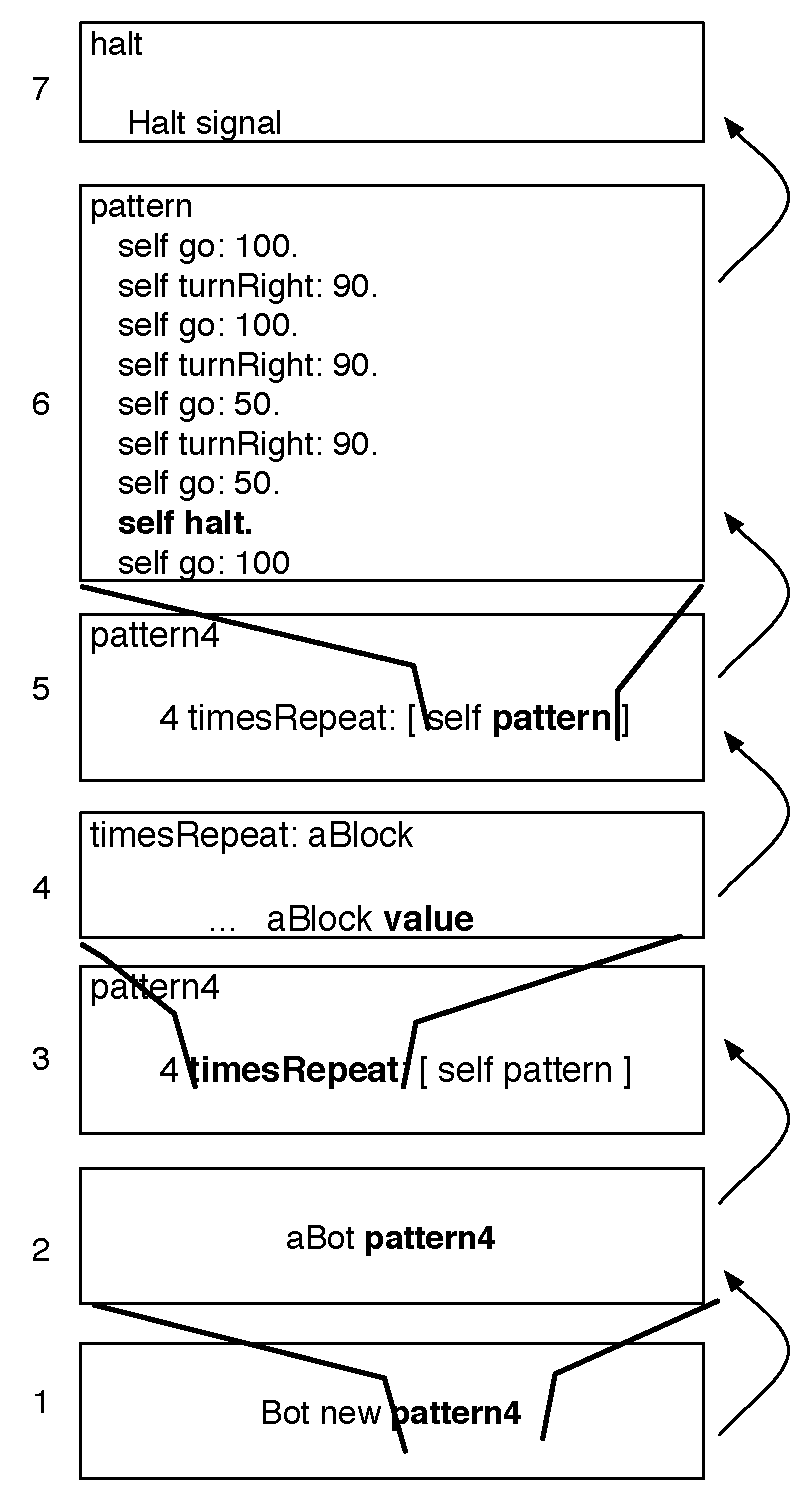
\includegraphics[width=7cm]{executionStack}
%\caption{The execution stack containing all the messages and the methods invoked resulting of the execution of \ct{Bot new pattern4}.  \label{fig:executionStack}}
%\end{figure}
\end{minipage}

@@Production: I want a number for the figure and the following caption: The execution stack containing all the messages and the methods invoked resulting of the execution of \ct{Bot new pattern4}.@@ 





\section{A First Look at the Debugger}

Right now you have imagined the sequence of messages sent and methods executed resulting from the execution of a message, but \sq has a debugger, a powerful tool that lets you see, navigate and change the chain of messages. The debugger is automatically invoked when a message is not understood by an object as I will show later, but you can invoke it explicitly by introducing the expression \ct{self halt} in the body of a method. Introducing such an expression is useful to understand or find a bug in a program. 

\cadre{A debugger is a tool that allow you to navigate through the executed methods.  Using a debugger, you can print the values of the argument, modify the method definition and continue to execution.}

To open a debugger, add the expression \ct{self halt} in the method \ct{pattern} as shown by method~\ref{selfhalt}. Then execute the expression \ct{Bot new pattern4}, you should obtain the situation depicted by Figure~\ref{fig:1DebuggerPatternHaltAnnotated}. A new robot is created, it started to draw the first pattern and got stopped and you get a chance to open a debugger. 

\begin{method}\label{selfhalt}
pattern 
   "draws a pattern"

   self go: 100.
   self turnRight: 90.
   self go: 100.
   self turnRight: 90.
   self go: 50.
   self turnRight: 90.
   self go: 50.
   \textbf{self halt.}
   self turnRight: 90.
   self go: 100.
   self turnRight: 90.
   self go: 25.
   self turnRight: 90.
   self go: 25.
   self turnRight: 90.
   self go: 50
\end{method}

\begin{figure}[h]
\centerline{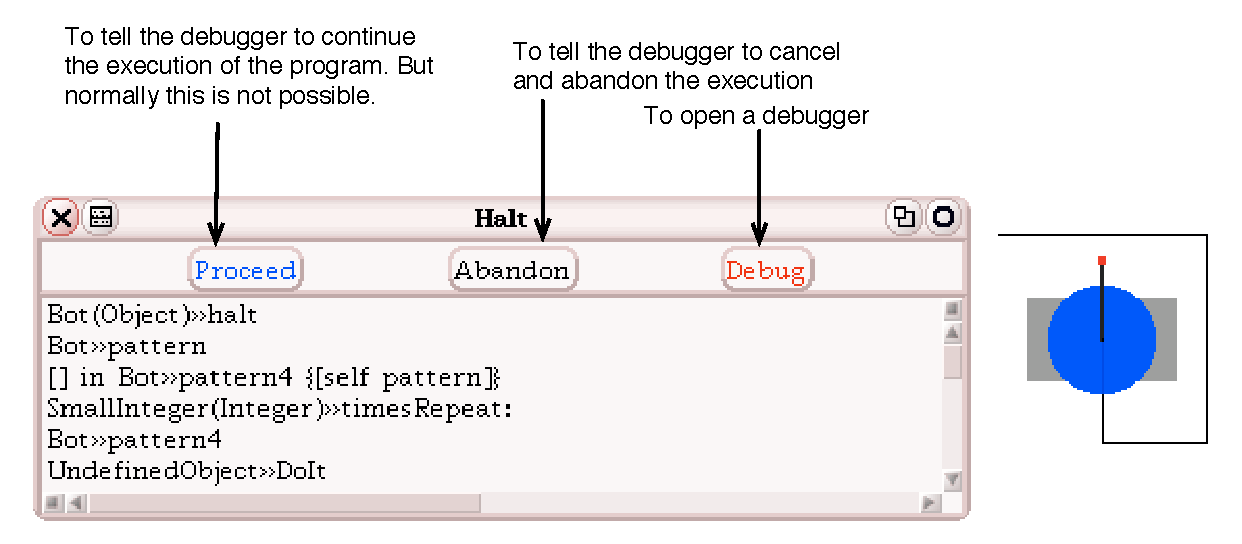
\includegraphics[width=10cm]{1DebuggerPatternHaltAnnotated}}
\caption{The robot started to draw the beginning of the first pattern then stopped and  you get a chance to open a debugger. \label{fig:1DebuggerPatternHaltAnnotated}}
\end{figure}



\cadre{To raise a debugger insert the expression \ct{self halt} in a method. The execution of the expression \ct{self halt} raises a debugger.}



The window presented in Figure~\ref{fig:1DebuggerPatternHaltAnnotated} proposes three buttons: \button{Proceed}, \button{Abandon} and \button{Debug}. 
\begin{itemize}
\item \textbf{Proceed.} This button tells the debugger to continue the execution of the message as if the self halt was not in the method. Note that this functionality is possible only if you provoked the error using \ct{self halt}. When it is a real error that raises the debugger, using proceed does not help since \sq cannot continue. 

\item \textbf{Abandon.} This button tells the debugger to simply close and it discards the actual execution. 

\item \textbf{Debug.} This button tells the debugger to open as shown by Figure~\ref{fig:2DebuggerPatternWithHaltPatternAnnotated}
\end{itemize}

If you press the \button{debug} and select the second line of the top pane, you obtain Figure~\ref{fig:2DebuggerPatternWithHaltPatternAnnotated}. The debugger is composed of several panes.  The top pane represents the execution stack that I presented in the first section: you get all the messages that have been sent just before the halt occurs, the most recent message on top. The most recent message is \ct{halt} therefore it is at the top of the stack and this is the the one that lead to the opening of the dialog box shown in Figure~\ref{fig:2DebuggerPatternWithHaltPatternAnnotated}.

\begin{figure}[h]
\centerline{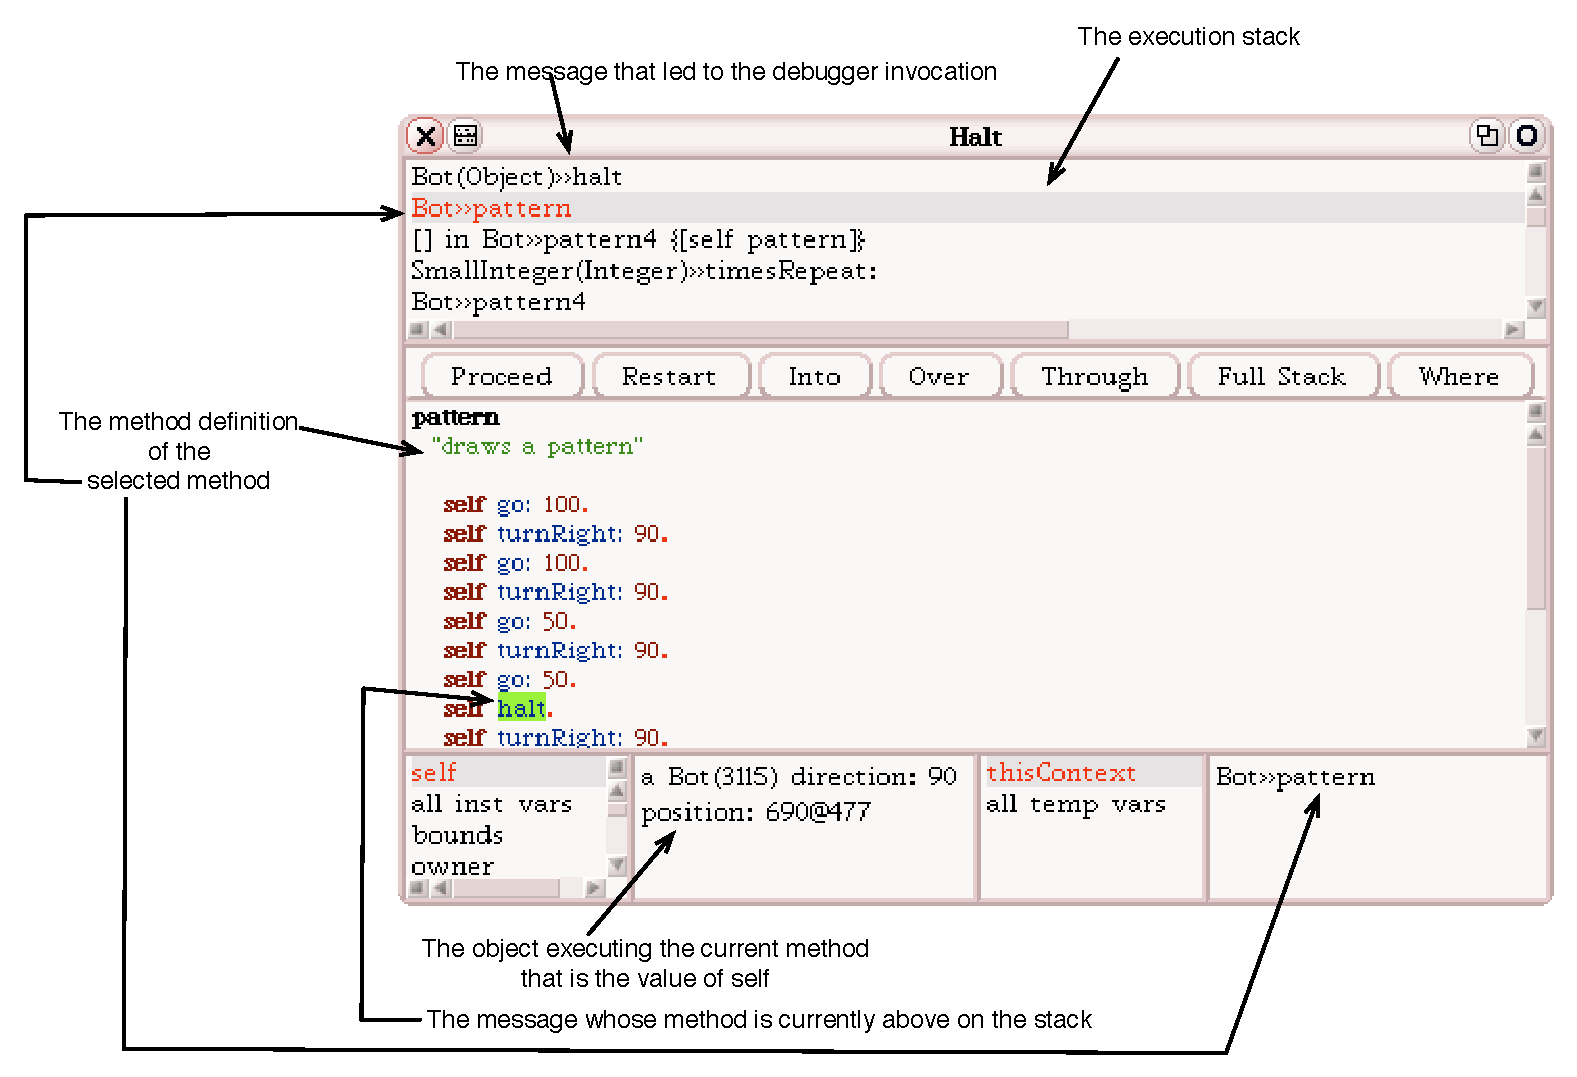
\includegraphics[width=10cm]{2DebuggerPatternWithHaltPatternAnnotated}}
\caption{Selecting the method \ct{pattern}. \label{fig:2DebuggerPatternWithHaltPatternAnnotated}}
\end{figure}

Selecting one of the lines in the top pane shows the method definition in the second pane.  Figure~\ref{fig:2DebuggerPatternWithHaltPatternAnnotated} shows that we selected the method \ct{pattern} in the stack, and its definition is shown in the second large pane. The object that received the message (that is the object referred to by the variable \ct{self}) and that executed the method \ct{pattern} is shown in the left bottom part. 

In the method body of the currently selected method, here \ct{pattern},  the debugger highlights in green the method whose execution is currently stopped and that is above the selected method on the stack. Here \ct{self halt} is currently stopped and then above \ct{pattern}. This also means that the expression above the self halt in the method body have been executed, while the one below haven't. Here \ct{self go: 100. self turnRight: 90. self go: 100. self turnRight: 90.} have already been executed. 

\begin{figure}[h]
\centerline{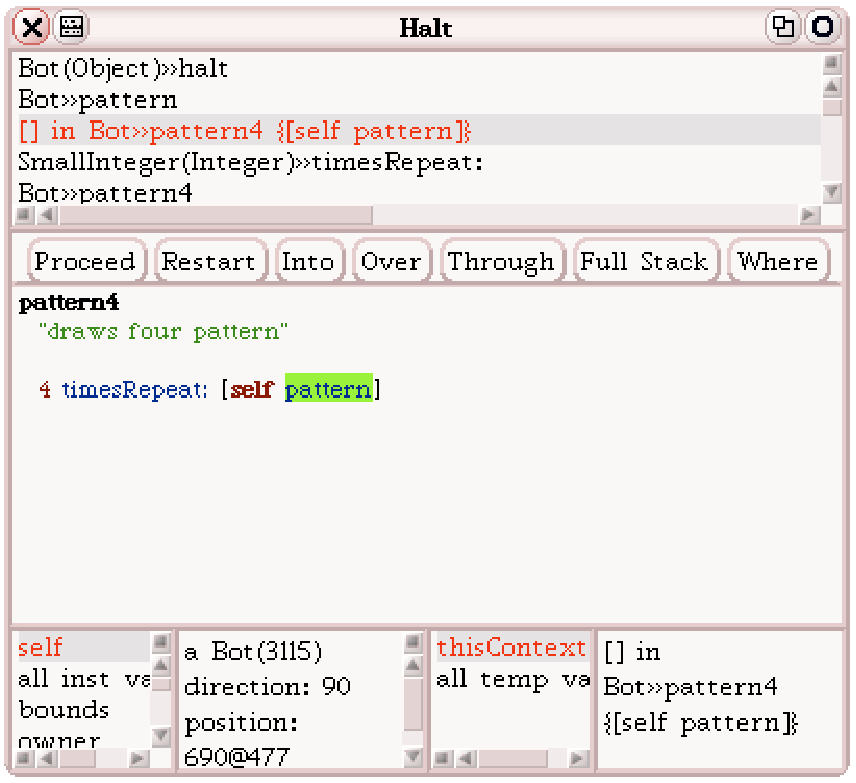
\includegraphics[width=7cm]{3DebuggerPattern}\hfill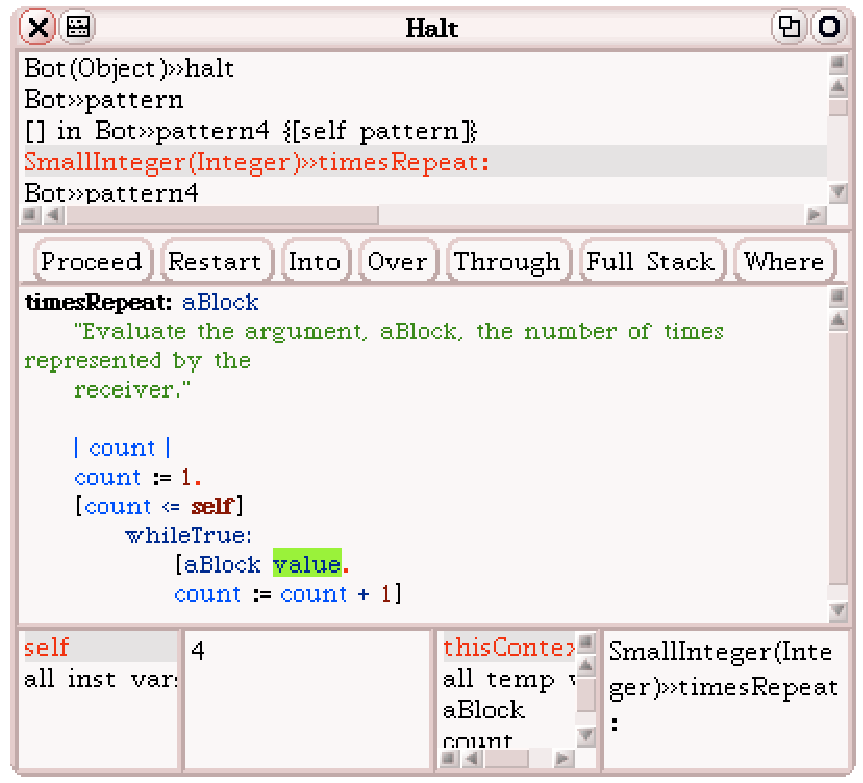
\includegraphics[width=7cm]{4DebuggerPatternTimesRepeat}}
\caption{Left: Selecting the method \ct{pattern4}. Right: Selecting the method \ct{timesRepeat:} \label{fig:3DebuggerPattern}}
\end{figure}


If you click on the third line, that is the method \ct{pattern4} you see that the stack of method execution above is related to the execution of the expression \ct{self pattern} of the method \ct{pattern4} (in Figure~\ref{fig:3DebuggerPattern}). Now if you click on the fifth line, you have a look again at the method \ct{pattern4} but before the loop is executed. The debugger indicates that the method above is related to the execution of the complete loop, \ct{timesRepeat: [ self pattern ]}. 

If you select the fourth line as shown in Figure~\ref{fig:3DebuggerPattern} you get the definition of the method \ct{timesRepeat:} itself. Again the debugger shows the  methods that are executed and lead to the method above in the stack. In addition notice that the object receiving the message is different, here this is not a robot but an integer as in the expression \ct{4 timesRepeat: [ self pattern ]} the receiver of the loop is the integer 4. This means that within this method the variable \ct{self} is bound to an integer. In fact this is normal as the variable self \emph{always} represents the object that received the current message. 

\section{Stepping in the Stack}
The \sq debugger not only lets you navigate the stack and identify the receiver of the messages, but it lets you execute step by step the method. You can ask the debugger to perform several actions using the buttons between the first and second pane. I describe the most useful ones from left to right.


\begin{figure}[h]
\centerline{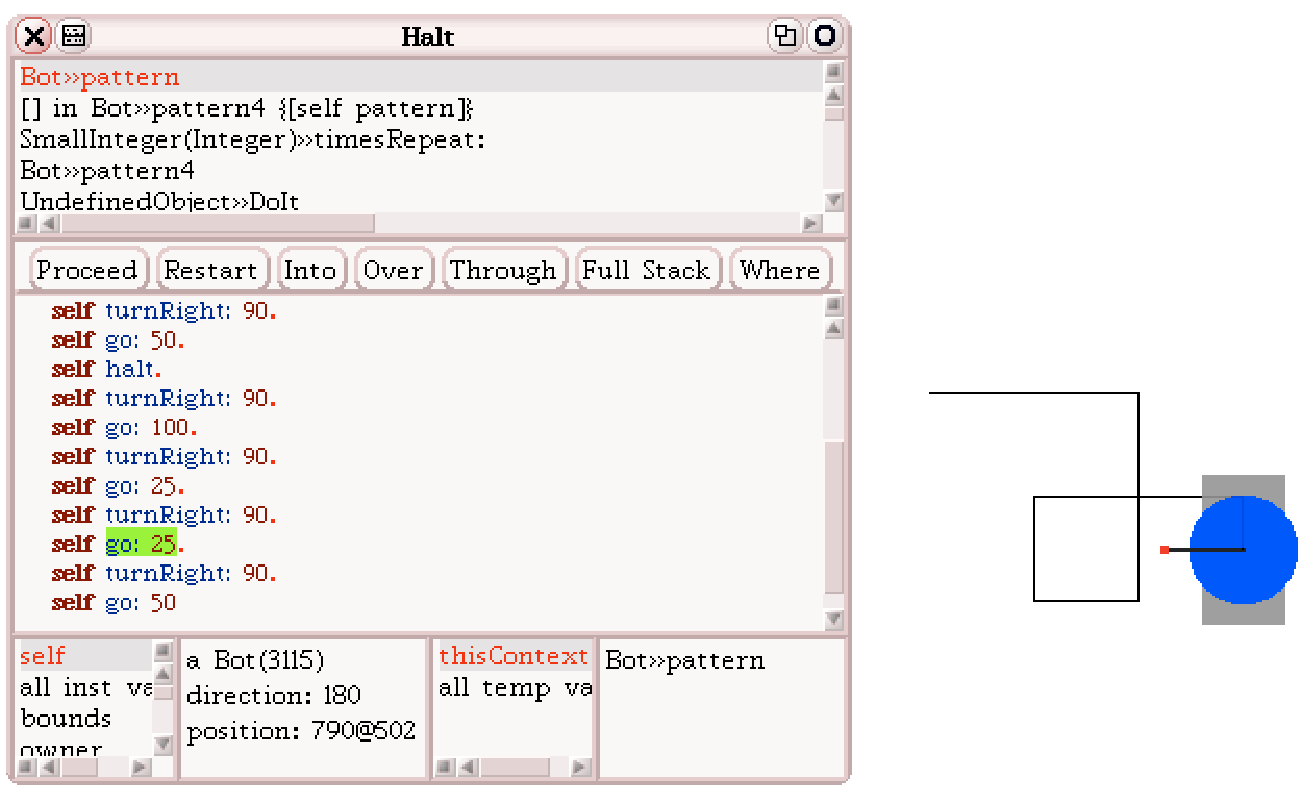
\includegraphics[width=10cm]{5DebuggerSteppingOverWithRobot}}
\caption{Stepping in the method \ct{pattern4} and seeing the robot executing all the stepped methods one by one.  \label{fig:4DebuggerPattern}}
\end{figure}

\begin{itemize}
\item \textbf{Proceed.} Pressing the button proceed as the same effect as pressing the button proceed in the dialog box shown in Figure~\ref{fig:1DebuggerPatternHaltAnnotated}: it closes the debugger and continues the method execution if possible.

\item \textbf{Restart.} You can ask the debugger to restart the execution of the current method. Note that sometimes this does not make sense since you may modify twice the same object and this may be incompatible. 

\item \textbf{Into.} Lets you go \emph{into}  the method currently selected without executing (See Figure~\ref{fig:5DebuggerPattern}). 

\item \textbf{Over.} This functionality is with the previous one the most used and useful of the debugger. It lets you execute the message currently selected but without going into the method execution. You simply execute the following expression and stop after. (See Figure~\ref{fig:4DebuggerPattern}). If you step over some expressions in the method \ct{pattern} you should see the robot performing each action one after the other.
Note that when you arrive at the end of the method, stepping over just return to the method that invokes the current one: you go down the stack. If you were stepping in \ct{pattern} then you would end up in \ct{pattern4}. 
\end{itemize}



When you press the button \button{Into}, you ask the debugger to go into the method without executing it. For example, if the currently selected expression in the method \ct{pattern} is \ct{self turnRight: 90}, then pressing the button \button{Into} asks the debugger to go inside the method \ct{turnRight:}, stopping at its first expression as shown by Figure~\ref{fig:5DebuggerPattern}. Here the first message to be sent is the message \ct{negated}. Again here you have the choice to go into the first expression or to execute it. Again when you reach the end of  a method, you come back to its calling method. Note that you can also see the value of the arguments passed to the method  by selecting the argument name on the method body and using print it (see Figure~\ref{fig:Argument}). 

\begin{figure}[h]
\centerline{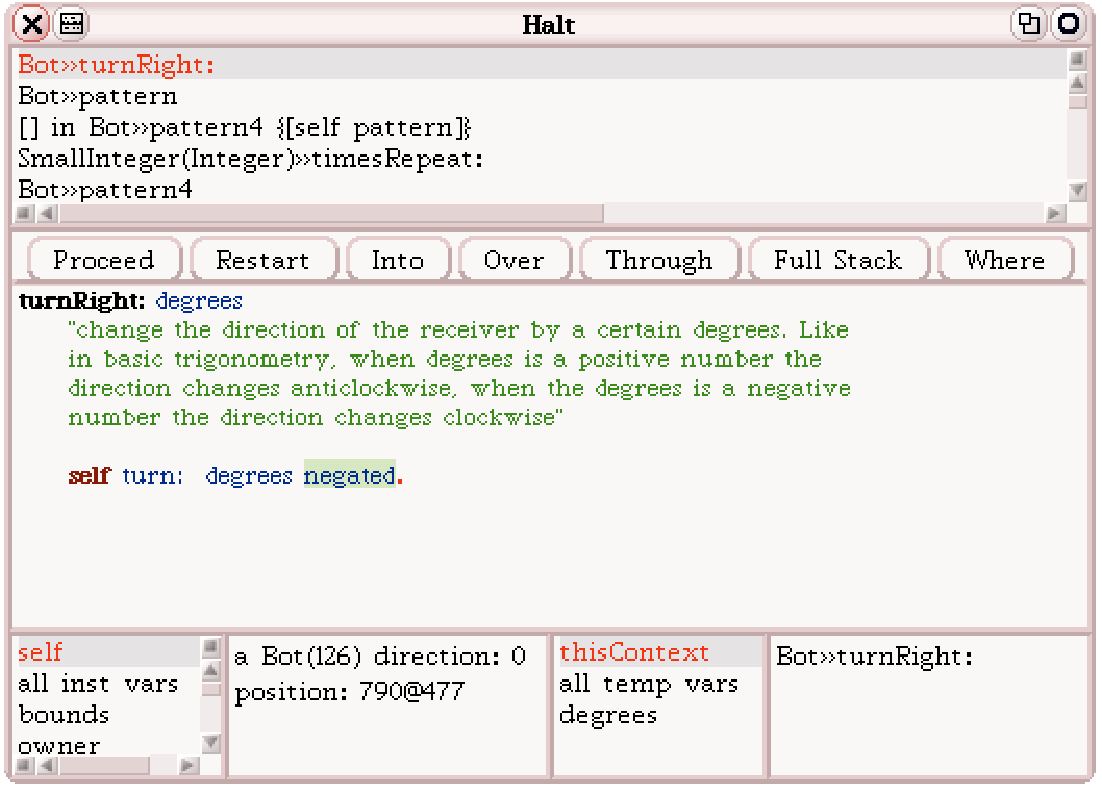
\includegraphics[width=7cm]{6DebuggerSteppingInto}}
\caption{Stepping into the method \ct{turnRight:} \label{fig:5DebuggerPattern}}
\end{figure}

\begin{figure}[h]
\centerline{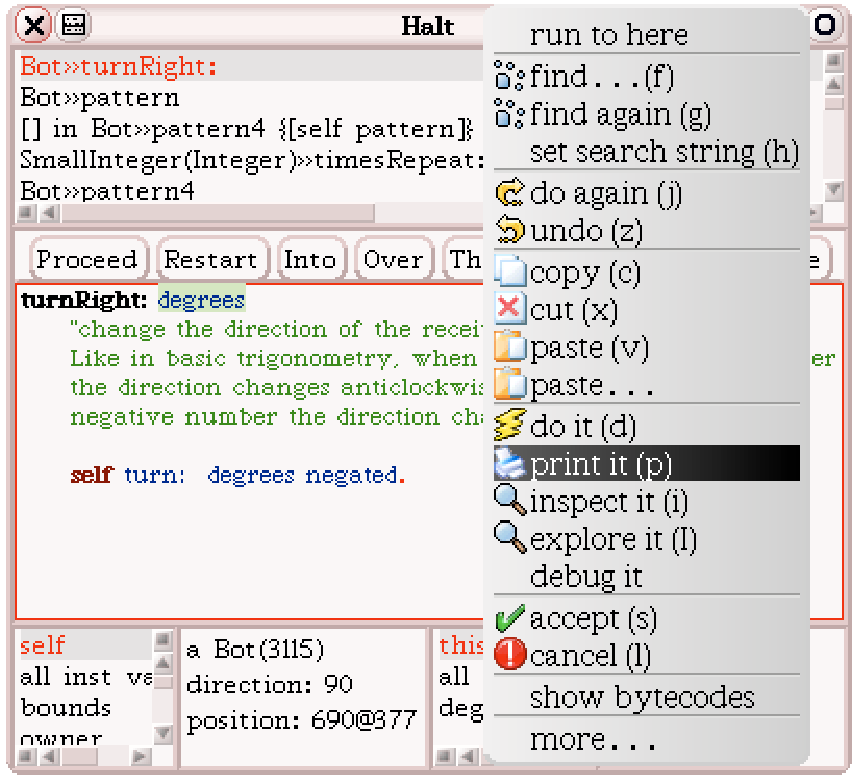
\includegraphics[width=7cm]{ArgumentSelected} 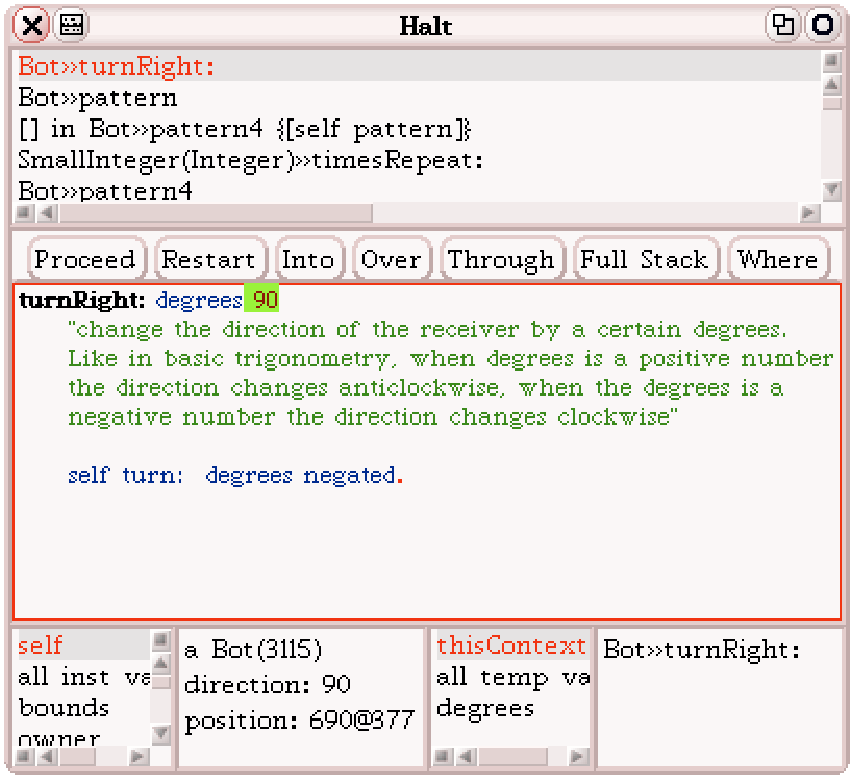
\includegraphics[width=7cm]{ArgumentPrinted}}
\caption{Right: Selecting an argument and printing. Left: Value printed. \label{fig:Argument}}
\end{figure}

In addition you can \emph{modify} the method definition inside the debugger by editing the code in place and accepting it via the contextual menu item \button{accept} (see Figure~\ref{fig:6DebuggerPattern}). For example in Figure~\ref{fig:5DebuggerPattern}, I restarted the method by pressing the \button{Restart} button then edited the method in the debugger itself and replaced the 100 of the first \ct{go:} message by \ct{500}. Then I recompiled the method by using the accept item choice of the menu. Now the robot will move 500 pixels if you press the \button{proceed} button.

\begin{figure}[h]
\centerline{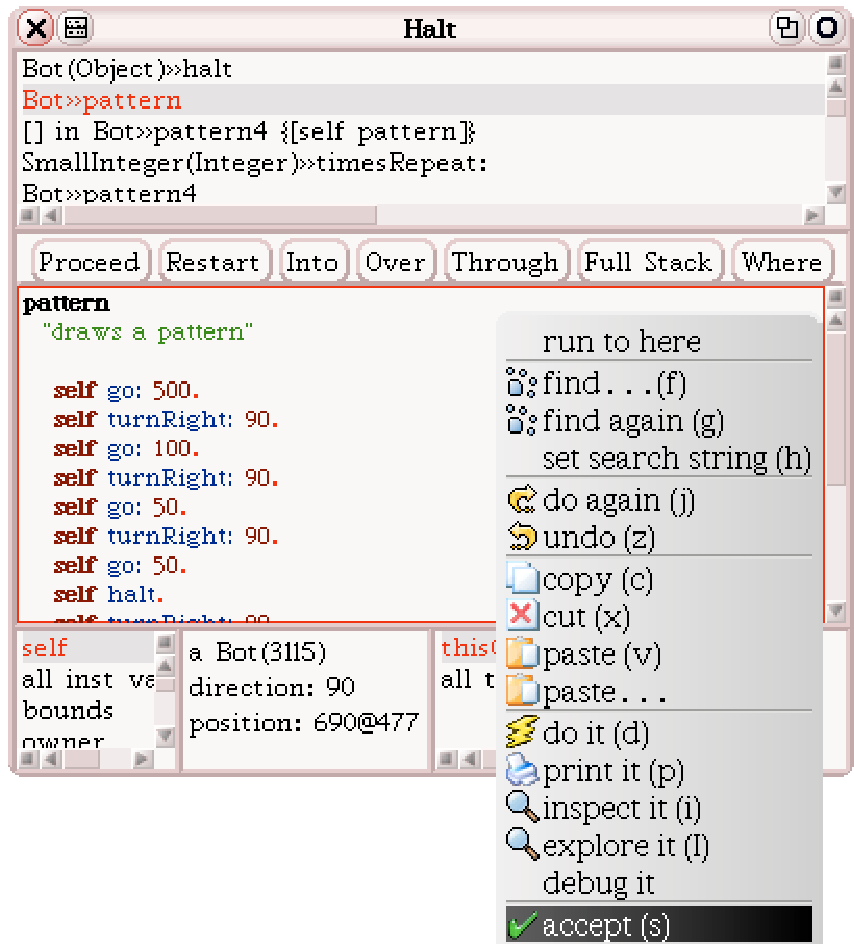
\includegraphics[width=7cm]{7DebuggerChangedValueA} 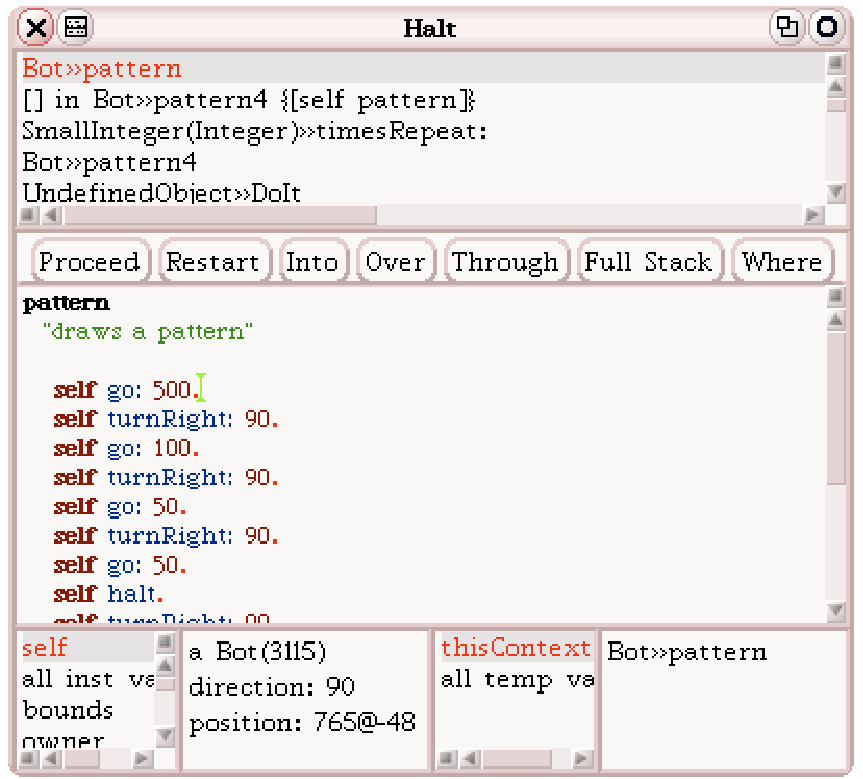
\includegraphics[width=7cm]{7DebuggerChangedValueB}}
\caption{Right: Editing the method definition and recompiling it. Left: Method \ct{pattern} recompiled\label{fig:6DebuggerPattern}}
\end{figure}

\section{Fixing Errors}
I show you that you can get a debugger by inserting the expression \ct{self halt} in the method. However, you can also use the debugger to fix your errors. When an object receives a message that it does not understand you can get a debugger. In fact when an object does not understand a message, \sq sends to this object the message \ct{doesNotUnderstand:} with a representation of the message. By default, the method \ct{doesNotUnderstand:} open a dialog box to ask you whether you want to get the debugger. You can use this debugger to navigate in the stack of  executed methods and try to understand what went wrong. 

\begin{figure}[h]
\centerline{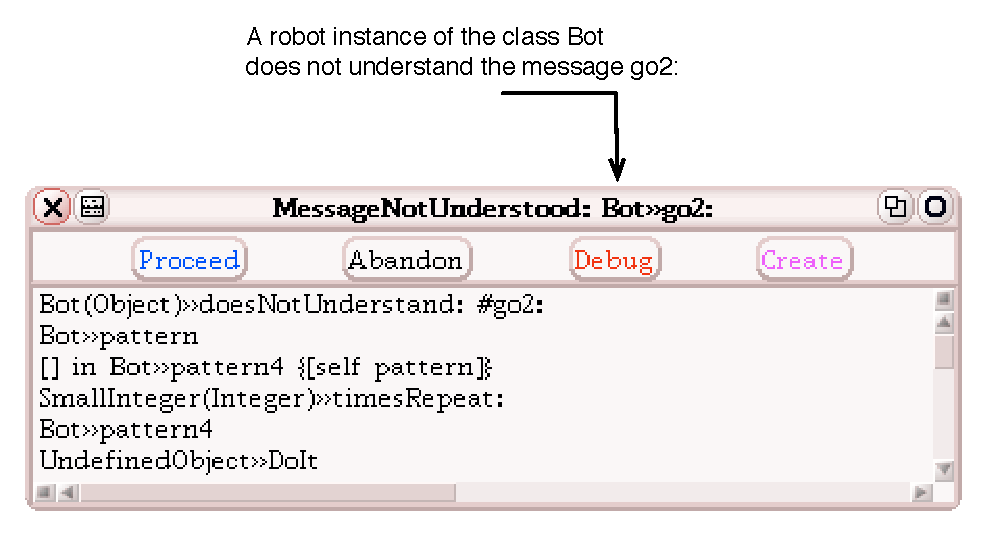
\includegraphics[width=7cm]{11DebuggerGo2Annotated} 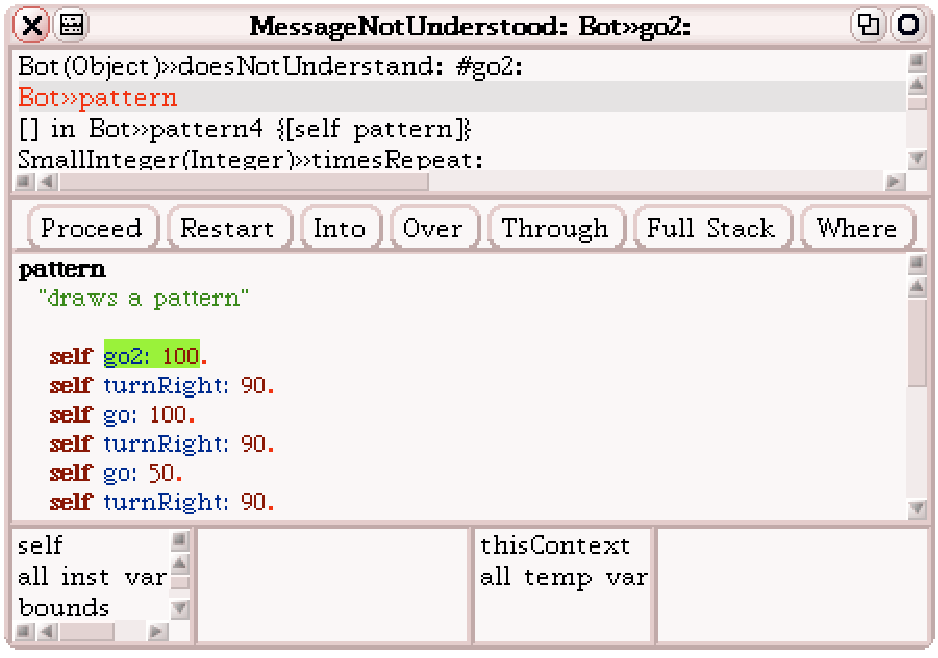
\includegraphics[width=7cm]{12DebuggerError}}
\caption{Left: Getting a \ct{doesNotUnderstand:} error. Right: Identifying the problem.\label{fig:11DebuggerGo2}}
\end{figure}


\paragraph{Example 1.} To illustrate the process, change the first line of the method \ct{pattern} to be \ct{self go2: 100} and  execute the expression \ct{Bot new pattern4}. You should get the debugger dialog box as shown in Figure~\ref{fig:11DebuggerGo2}.
The debugger dialog box indicates that the receiver, a robot created by the class \ct{Bot}, does not understand the message \ct{go2:}. When you press the button \button{Debug} of the dialog you get the debugger shown on the right of Figure~\ref{fig:11DebuggerGo2}.

The method on the top of the stack is the method \ct{doesNotUnderstand:} which is sent to the receiver of a message, when the receiver does not understand a message. The method directly below it is then the method containing the message leading to the error and the call of the method \ct{doesNotUnderstand:}. Here the method \ct{pattern} contains the message \ct{go2:} which is not understood by the robot as shown in Figure~\ref{fig:11DebuggerGo2}


\paragraph{Example 2.} 
Now change the first line of the method \ct{pattern} to be \ct{self go: nil} and  execute the expression \ct{Bot new pattern4}. You should get the debugger dialog box as shown in Figure~\ref{fig:8DebugAnotherError}. The error is more difficult to spot. 
Here, the dialog box title \ct{MessageNotUnderstood: UndefinedObject} indicates that there is a message not understood sent to \ct{nil}, which is an instance of the class \ct{UndefinedObject}.


\begin{figure}[h]
\centerline{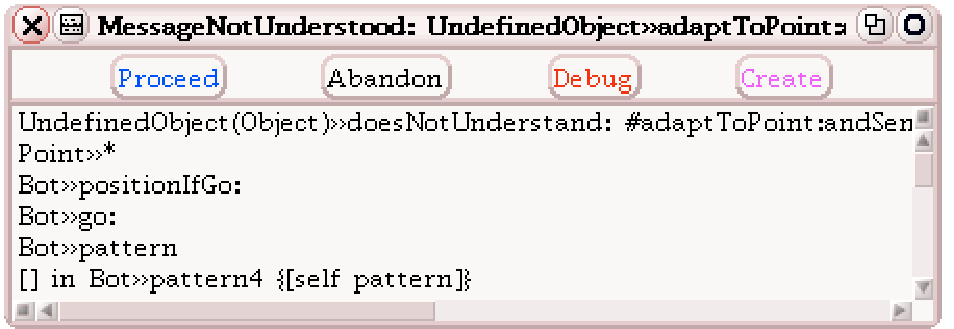
\includegraphics[width=7cm]{8DebugAnotherError}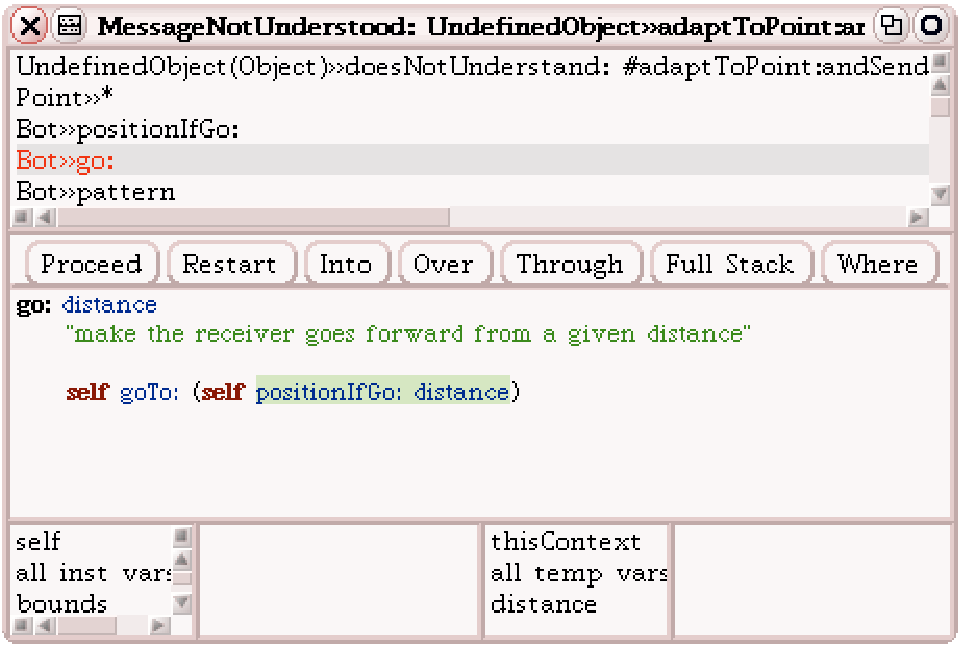
\includegraphics[width=7cm]{8bDebugAnotherError}}
\caption{Left: A message not understood sent to \ct{nil}. Right: Going down the execution stack. \label{fig:8DebugAnotherError}}
\end{figure}

The fact that \ct{nil} was passed as value led to an error after several other method executions. Therefore you have to go down the stack to the point where you can understand your mistake and fix it. For example, in Figure~\ref{fig:8DebugAnotherError} right, the second method from the top shows that something wrong happened with \ct{*}, but the problem does not come from this method. This is the same situation in the following method. Select the method \ct{go:}, you can see that the method \ct{go:} just passes the argument it gets from the method \ct{pattern} to the method \ct{positionIfGo:}. If you select the parameter \ct{distance} and print its value you get \ct{nil}. This indicates 
that the problem comes from a place further down the stack. 

\begin{figure}[h]
\centerline{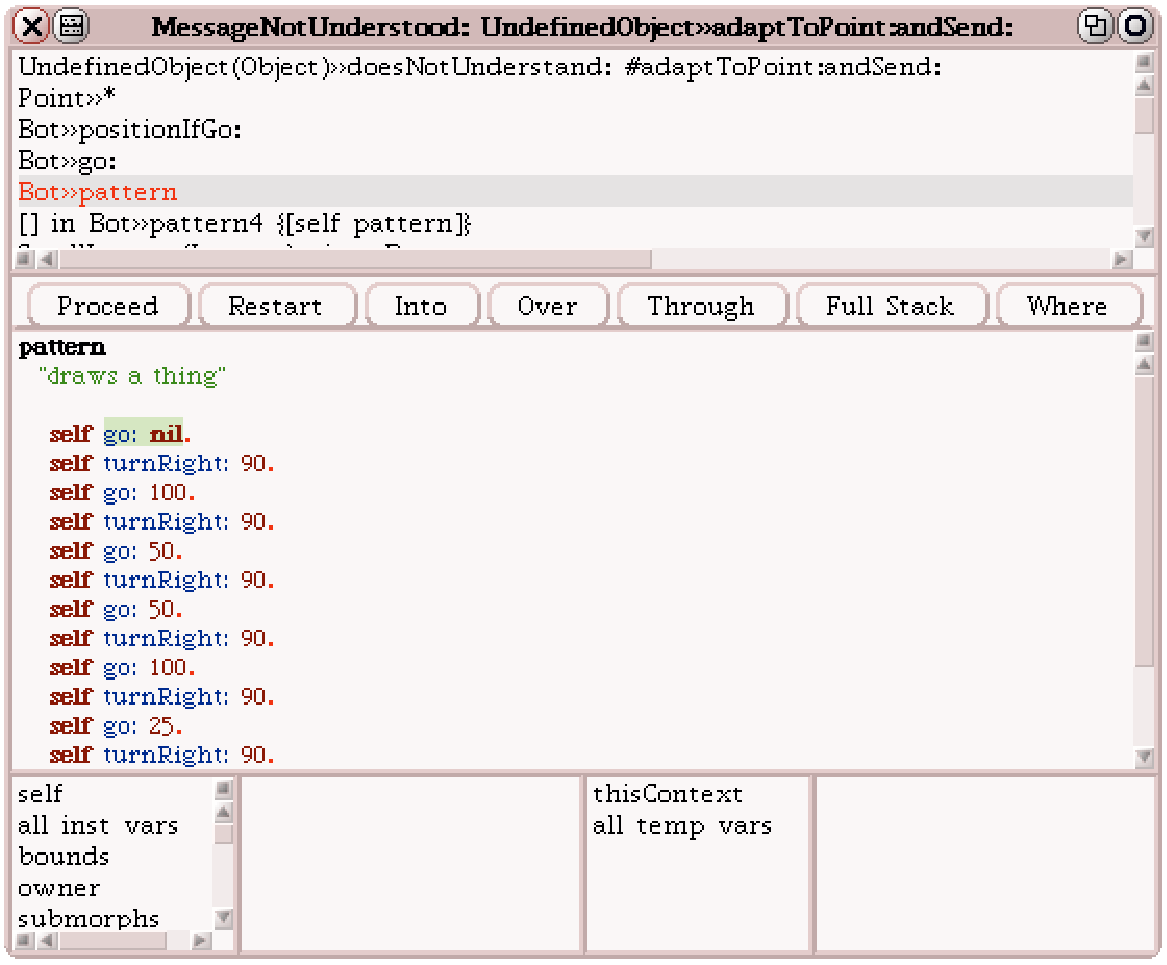
\includegraphics[width=7cm]{9DebugAnotherErrorFinding} 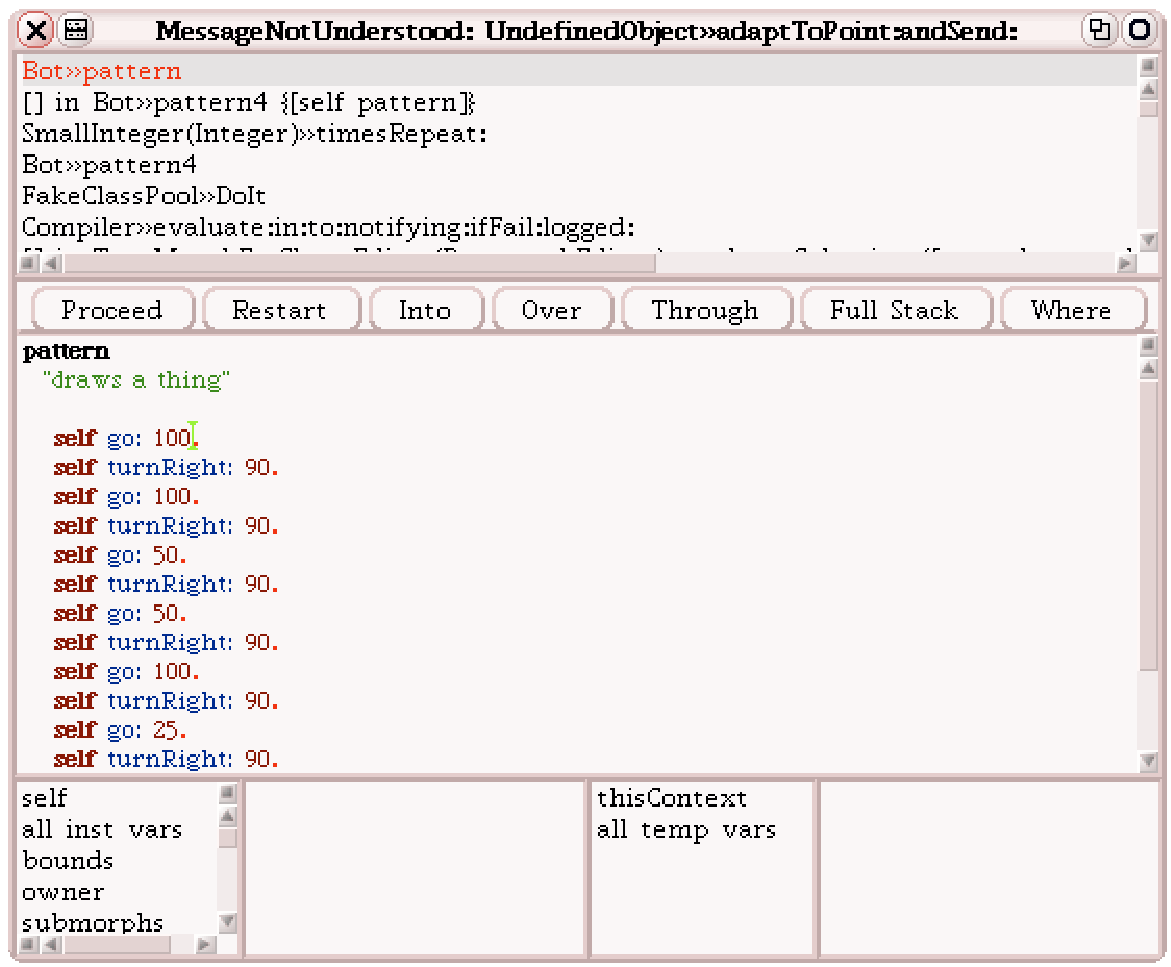
\includegraphics[width=7cm]{10RecompilingMethod}}
\caption{Left: Editing the method definition and recompiling it. Right: Method \ct{pattern} recompiled.\label{fig:9DebuggerPattern}}
\end{figure}


Finally as shown in Figure~\ref{fig:9DebuggerPattern} left, you see that \ct{nil} is passed as argument instead of a number as expected by the method \ct{go:}. You can now fix the bug by editing the method \ct{go:} and replacing \ct{nil} by the value, and press the button \button{Proceed} to let the execution runs. 

Note that in this example, I use \ct{nil} to get a really simple problem to identify. While you can get this kind of bugs, you will have to face all kind of unexpected situations leading to a bug. However, the process is the same, you will use the debugger, navigate through the stack, check the values of the arguments until you understand what went wrong. You may be forced to change your code and not only the arguments of messages sent. 


\summa

\begin{itemize}
\item By default, in \st the value of a uninitialized variable is \nil. \nil is an object that represents undefined values, \ie objects with which we cannot do too much, hence leading to error.

\item A debugger is a tool that allow you to navigate through the executed methods. Using a debugger, you can print the values of the argument, modify the method definition and continue to execution.

\item To raise a debugger insert the expression \ct{self halt} in a method. The execution of the expression \ct{self halt} raises a debugger. 
\end{itemize}










%
%\section{Understanding Error with the Debugger}
%I would like to show you how you can find errors. For that any \st system contains a debugger \ie a tool that lets us look at the way messages are executed and change them. In this section, we just want to give you an overview and be sure that you are not afraid by the debugger.

%
%\begin{figure}[h]
%\centerline{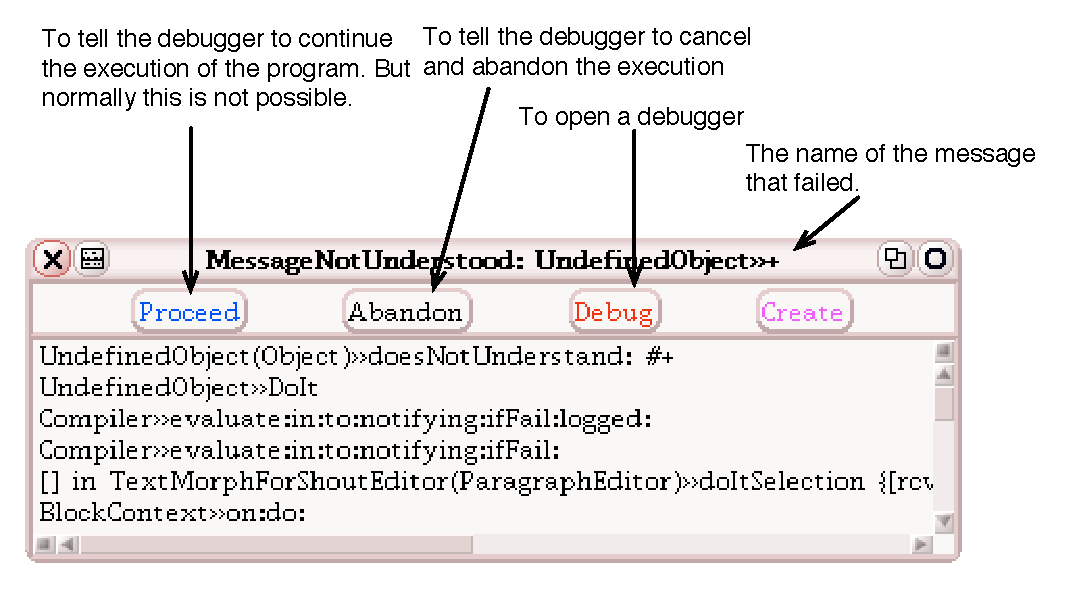
\includegraphics[width=10cm]{debuggerOneAnnotated}}
%\caption{When an error occurs a window invites us to open a debugger.\label{fig:plusDonotUnder}}
%\end{figure}

%If you answer \emph{yes} to the question that \sq asks when executing the script~\ref{scr:uninitSizeplus10} \sq attempts to send the message "\ct{+\ 10}" to the object \ct{nil}. Of course, this message is not understood by \nil. \nil understands a very limited set of messages, so a debugger window opens on the screen (see Figure~\ref{fig:plusDonotUnder}). Note that a similar problem can occurs if you initialized the value with something else than a number. So the process of finding the error is similar.  

%%The window presented in Figure~\ref{fig:plusDonotUnder} propose four buttons: \button{Proceed}, \button{Abandon} and \button{Debug}. 
%%\begin{itemize}
%%\item \textbf{Proceed.} This button tells the debugger to continue the execution of the message. Note that this functionality is possible only if you provoked the error using some specific messages. In the context of this book you will normally not be able to use this functionality. 
%%\item \textbf{Abandon.} This button tells the debugger to simply close.
%%\item \textbf{Debug.} This button tells the debugger to open as shown by Figure~\ref{fig:debug1Debug}.
%%\item \textbf{Create.} This button create an empty method in the class of the receiver. We do not cover the functionality of this button in this book.
%%\end{itemize}

%Notice that the window label indicates also the message in which the error occurred, here we get to know that the error occurred while trying to execute the message \ct{+}. Note that the information below the three button is clearly not comprehensible by normal humans, therefore we suggest you to do not pay attention to it.

%

%If you press the \button{debug}, you obtain Figure~\ref{fig:debug1Debug}. The debugger is composed of several panes.  The top pane represents the sequence of all the messages that have been sent just before the error occurs, the most recent message on top. This sequence is also called an \emph{execution stack}. Selecting one of the lines in the first pane shows the method definition of the code of the message sent in the second pane, as shown in the Figure~\ref{fig:debug1sizenil}. Figure~\ref{fig:debug1sizenil} shows that we selected another message in the stack. It shows the new selected message, here Doit, as we asked to execute a script and the code of its definition, here it just shows the script itself. More important the debugger shows some other information like the value associated with the variable \ct{size}. 

%
%\begin{figure}[h]
%\centerline{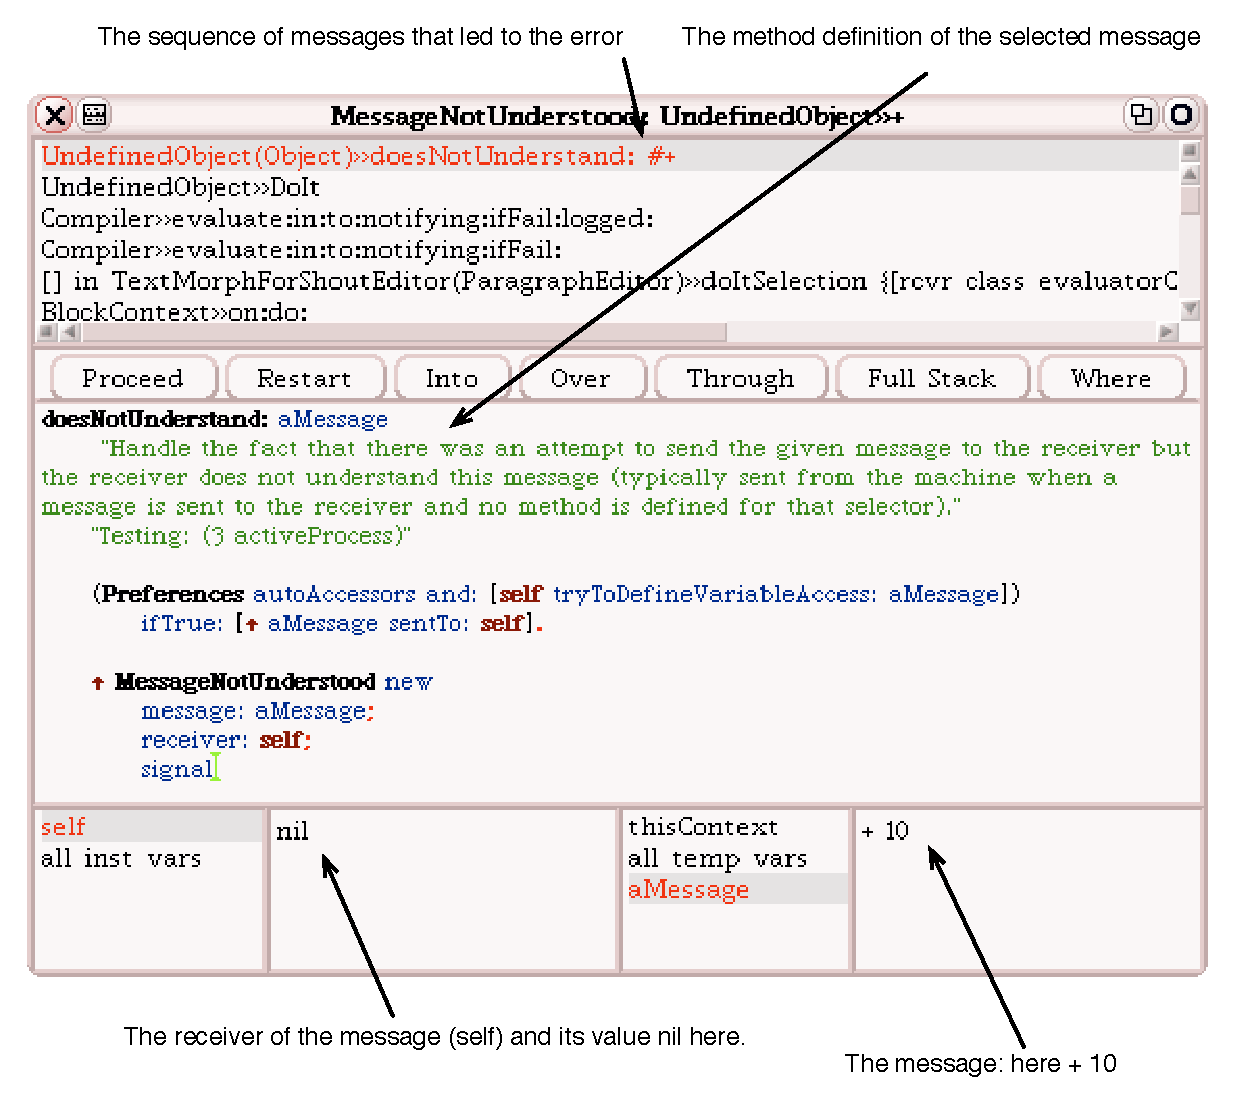
\includegraphics[height=8cm]{debuggerTwoAnnotated}}
%\caption{Debugger window active just starting to debug.\label{fig:debug1Debug}}
%\end{figure}

%

%
%Note that as \ct{+} was sent to the variable \ct{size}, \ct{self} the receiver of the message also represents it(see Chapter~\ref{ch:turtleTeaching}). Here both \self and \ct{size} have \nil as value. To see it, just click on \self in the left bottom pane or just click on the variable \ct{size} on the right bottom part of the debugger. 

%We will not introduce all the buttons of the debugger at this point as we would have to go in too much detail for now. However, there is still one last point that we want to show you. If you change the value associated with the variable \ct{size} by editing the rightmost bottom pane with the new value and accepting it. In Figure~\ref{fig:debuggerFourAnnotated} we assigned 100 to the variable \ct{size}. Once you changed the value of the variable, you can select for example \ct{size + 10} in the middle pane and print it and you will get the expected value. 

%
%\begin{figure}[!h]
%\centerline{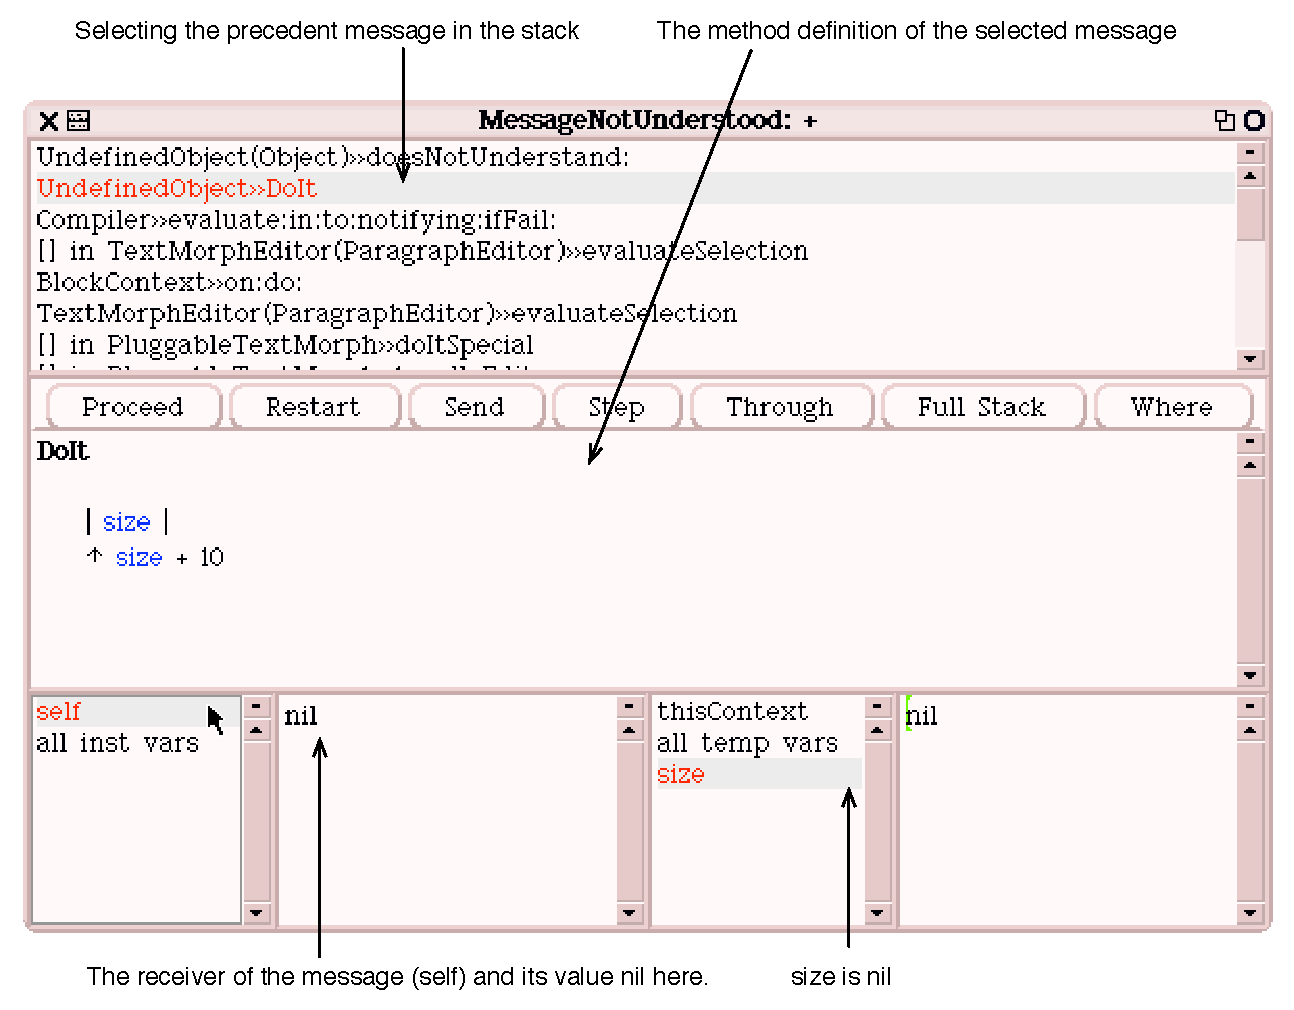
\includegraphics[height=8cm]{debuggerThreeAnnotated}}
%\caption{Debugger window occurring when attempting the execution
%of a message unknown to an object.\label{fig:debug1sizenil}}
%\end{figure}

%\begin{figure}[!h]
%\centerline{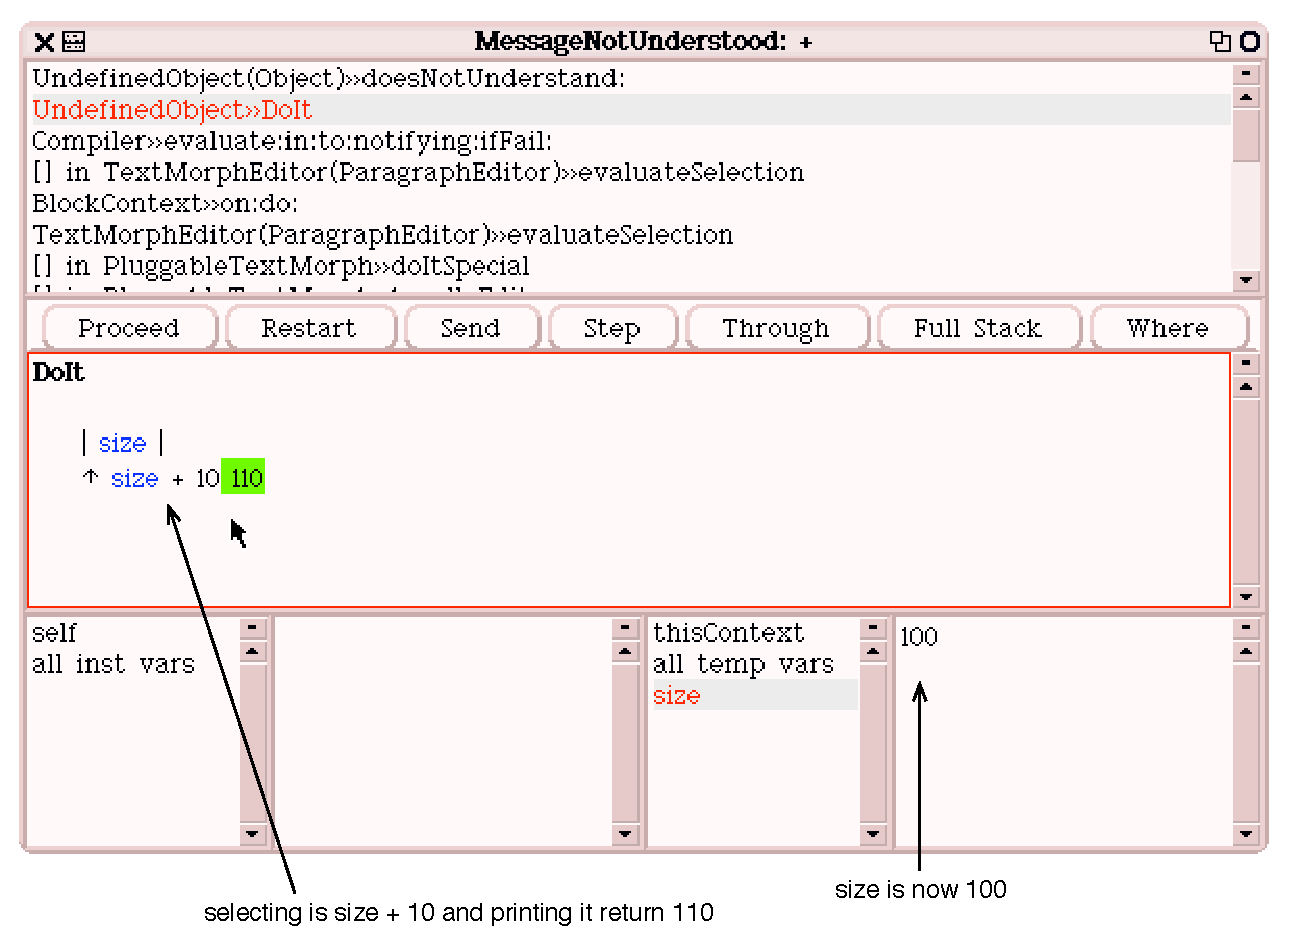
\includegraphics[height=8cm]{debuggerFourAnnotated}}
%\caption{Once a variable value is modified you can execute expressions.\label{fig:debuggerFourAnnotated}}
%\end{figure}

%Finally we want to show that you can navigate and follow the messages that led to an error. Execute the script~\ref{exemplepasvar} and open a debugger.

%\begin{scriptwithtitle}{Broken script}\label{exemplepasvar}
%| caro size | 
%caro := Turtle new.  
%caro go: size.
%\end{scriptwithtitle}

%What you should understand is that a wrong value for a variable propagates from the place that originates until the place where it actually breaks the execution of a message. So often the first message on the stack is not really interesting. While browsing in the stack you can understand where the error comes from and find finally the place where the mistake was initiated. For example, the first debugger in Figure~\ref{fig:debuggerFive}, tells us that the execution of the method \ct{adaptToPoint:andSend:} failed. We do not know anything of this method so we try to see who calls it. 

%When you select another message on the stack, the debugger highlights in green the expression that was executed and participated to the message that led to the error. For example, if you select the message \ct{go:}, you will see that the debugger indicates that the error occurred while executing the expression \ct{self positionInDirectionForDistance: distance} as shown by the second debugger. The third debugger shows that size was not initialized. However, when you will learn in Chapter~\ref{ch:turtleTeaching} to define methods that call other ones, you will see that errors are not only in the script but in method definitions too. 

%\begin{figure}[!h]
%\begin{center}
%\includegraphics[height=6cm]{debuggerFive}\includegraphics[height=6cm]{debuggerSix}
%\includegraphics[height=6cm]{debuggerSeven}
%\caption{Navigating through the messages.\label{fig:debuggerFive}}
%\end{center}
%\end{figure}





%The key thing to understand variables is to know that the variable name always refers to the \emph{value} associated with the variable, except if the variable is on the left of the construct \ct{:=}. In this case the variable name represents the placeholder itself containing the variable value and not the variable value itself.

%We also say that the value of a variable is always read, except when it appears on the left of \ct{:=} where it is written.

\ifx\wholebook\relax\else\end{document}\fi
